%Created on: Dec 21, 2017        Created by: P.Gimby

%Template for standard lab

% Beginning code for all standard physics latex documents

%Created on: May 8, 2014    Edited by: Wesley Kyle
%Edited on:	May 12, 2016	Edited by: P. Gimby - cleaned up the code to remove unneeded packages
%Edited on:	May 13, 2016	Edited by: P. Gimby - collected a few more packages used in 325.
%Edited on:	May 16, 2016	Edited by: P. Gimby - fixed page numbering error.
%Edited on: May 20, 2016	Edited by: Alex Shook - Added packages for 497

\documentclass[justified]{tufte-book}
\usepackage{graphicx} % allow embedded images
\setkeys{Gin}{width=\linewidth,totalheight=\textheight,keepaspectratio}
\usepackage{amsmath}  % extended mathematics
\usepackage{bm}  % bold font in math mode
\usepackage{longtable} %lets long tables flow into multiple pages instead of running off the page or having to break tables up manually
\usepackage{booktabs} % book-quality tables
\usepackage{units}    % non-stacked fractions and better unit spacing
\usepackage{multicol} % multiple column layout facilities
\usepackage{tikz} %for drawing nice pictures
\usepackage{indentfirst} % makes first line of each new section be indented
\usepackage{enumitem} % extended options for the enumerate environment
\usepackage{soul} % gives more typestting options like spacing, underline, and strike-through
\usepackage{marvosym} %extra symbols package
\usepackage{multirow} % for special table controls
\usepackage[singlelinecheck=false]{caption} % allow captions w/o figure number
\captionsetup{compatibility=false} % corrects in issue with the caption package
\usepackage{float} % allows for contorl over position of figures and tables
\allowdisplaybreaks % allows equations to span two pages if needed
\usepackage{mathrsfs} % fancy math symbols
\usepackage{multirow} % for special table controls
\usetikzlibrary{arrows,shapes,snakes,calc,patterns,3d} % addon to tikz
\usetikzlibrary{circuits.ee.IEC} % addon to tikz
\usepackage{pgfplots} % package for making plots of functions
\usepackage{gensymb} % symbols i,e. degrees
\usetikzlibrary{decorations.pathmorphing} % to draw the springs
\tikzset{circuit declare symbol = ac source}
\tikzset{set ac source graphic = ac source IEC graphic}
\usepackage{changepage} % allows for full page environment
\usepackage{comment} % allows comment tags for large sections

% define new page style that puts page numbers in the middle
%\begin{comment}
\fancypagestyle{custom}{
\fancyhf{} % clear all header and footer fields
\fancyheadoffset{0pt}
\fancyfootoffset{0pt}
\fancyfoot[C]{\thepage}
\renewcommand{\headrulewidth}{0pt}
\renewcommand{\footrulewidth}{0pt}}
\pagestyle{custom}
%\end{comment}

%below creates a new circuit symbol for AC sources
\tikzset{
         ac source IEC graphic/.style=
          {
           transform shape,
           circuit symbol lines,
           circuit symbol size = width 3 height 3,
           shape=generic circle IEC,
           /pgf/generic circle IEC/before background=
            {
             \pgftransformresetnontranslations
             \pgfpathmoveto{\pgfpoint{-0.8\tikzcircuitssizeunit}{0\tikzcircuitssizeunit}}
             \pgfpathsine{\pgfpoint{0.4\tikzcircuitssizeunit}{0.4\tikzcircuitssizeunit}}
             \pgfpathcosine{\pgfpoint{0.4\tikzcircuitssizeunit}{-0.4\tikzcircuitssizeunit}}
             \pgfpathsine{\pgfpoint{0.4\tikzcircuitssizeunit}{-0.4\tikzcircuitssizeunit}}
             \pgfpathcosine{\pgfpoint{0.4\tikzcircuitssizeunit}{0.4\tikzcircuitssizeunit}}
             \pgfusepathqstroke
            }
          }
        }
% end of circuit symbol
%\begin{document}
%%%end individual beginning code/,$d


%  \begin{titlepage}
%    \vspace*{\fill}
%    \begin{center}
%      \huge{{\bf TITLE1}}\\[0.4cm]
%      \huge{TITLE2}\\[0.4cm]
%      \LARGE{Laboratory Manual}\\[0.4cm]
%      \large{SEASON YEAR}
%    \end{center}
%    \vspace*{\fill}
%  \end{titlepage}
%\maketitle

%\begin{spacing}{0.5}
%\tableofcontents
%\end{spacing}

%NEW PHYS 497 PACKAGES AND COMMANDS

%Subcaption package: Allows subfigures to be placed side by side, and labeled with individual captions (Added June 1, 2016)
\usepackage{subcaption}

%Array package: Allows for addiation specifications in arrays (Added May 6, 2016)
\usepackage{array}

%newcolumntype: Allows one to specify a fixed column width (Added May 6, 2016)
\newcolumntype{L}[1]{>{\raggedright\let\newline\\\arraybackslash\hspace{0pt}}m{#1}}
\newcolumntype{C}[1]{>{\centering\let\newline\\\arraybackslash\hspace{0pt}}m{#1}}
\newcolumntype{R}[1]{>{\raggedleft\let\newline\\\arraybackslash\hspace{0pt}}m{#1}}

%circuits.logic.US, circuits.logic.IEC: For drawing logic gates in Tikz (Added May 6, 2016) 
\usetikzlibrary{circuits.logic.US,circuits.logic.IEC}

\newcommand{\PGT}{ %PGT: positive going transition
\begin{tikzpicture}
\draw[-angle 60] (0,0) -- (0,5pt);
\draw (0,5pt) -- (0,6pt) -- (5pt,6pt);
\draw (-5pt,0) -- (0,0);
\end{tikzpicture}
}





%TEST
\usepackage{geometry}
\pagestyle{fancy}

%\usepackage[caption=false]{subfig}

%\makeatletter
%\renewenvironment{figure}[1][htbp]{%
%  \@tufte@orig@float{figure}[#1]%
%}{%
%  \@tufte@orig@endfloat
%}

%\renewenvironment{table}[1][htbp]{%
%  \@tufte@orig@float{table}[#1]%
%}{%
%  \@tufte@orig@endfloat
%}
%\makeatother

% use instead of subfigure
\makeatletter
\newenvironment{multifigure}[1][htbp]{%
  \@tufte@orig@float{figure}[#1]%
}{%
  \@tufte@orig@endfloat
}
\makeatother

\makeatletter
\newenvironment{mainfigure}[1][htbp]{%
\@tufte@orig@float{figure}[#1]
\begin{adjustwidth}{}{-153pt}}
{\end{adjustwidth}\@tufte@orig@endfloat}%
\makeatother

\makeatletter
\newenvironment{maintable}[1][htbp]{%
\@tufte@orig@float{table}[#1]
\begin{adjustwidth}{}{-153pt}}
{\end{adjustwidth}\@tufte@orig@endfloat}%
\makeatother

%%%% Labatorial Cross-over labs need this code. This should be temporary PG Dec 7, 2016

\newcounter{questioncounter}
\setcounter{questioncounter}{0}
\newcounter{checkpointcounter}
\setcounter{checkpointcounter}{0}
\newcounter{figurecounter}
\setcounter{figurecounter}{0}
%%%%%%%%%%%%%%%%%%%%%%%%%%%%%%%%%%%%%%%%%%%%%%%%%%%%%%%

\newcommand{\checkpoint}{
 \fbox{\begin{minipage}{0.2\textwidth}
 %\includegraphics[width=0.5\textwidth]{stop}
 \end{minipage}
 \begin{minipage}{1.0\textwidth}
 {\bf CHECKPOINT \addtocounter{checkpointcounter}{1} \arabic{checkpointcounter}: Before moving on to the next part, have your TA check the results you obtained so far.}
 \end{minipage}}}

%%% end labatorial cross-over code.

% New environment for placing figure captions under the figure
%\makeatletter
%\newenvironment{mainfigure}{\textwidth}[1][htbp]{%
%\@tufte@orig@float{figure}[#1]%
%}{%
%\@tufte@orig@endfloat
%}
%\makeatother
 % uses tufte-book

\begin{document}

%%%start document%%% DO NOT REMOVE THIS LINE

\chapter{Creating Diagrams with TikZ}


\section{Plotting functions}


\begin{figure}
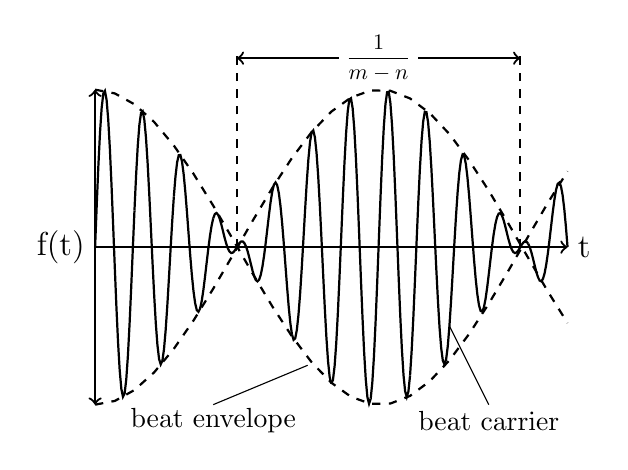
\begin{tikzpicture}

\draw[thick,<->] (0,-2)--(0,2); %yaxis
\draw[thick,->](0,0)--(6,0); %xaxis
\node[thick,left,font=\large] at (0,0){f(t)};
\draw[thick,dashed](1.8,0)--(1.8,2.5);
\draw[thick,dashed](5.4,0)--(5.4,2.5);
\draw[thick,<->](1.8,2.4)--(5.4,2.4);
\node[black,fill=white,shape=rectangle,scale=.8]at (3.6,2.4){$\dfrac{1}{m-n}$}; %beat freq
\node[thick] at (1.5,-2.2){beat envelope}; %envelope label
\node[thick] at (5,-2.2){beat carrier}; %carrier label
\node[thick,right,font=\large] at (6,0){t};
\draw(1.5,-2)--(2.7,-1.5);
\draw(5,-2)--(4.5,-1);

\draw[thick,domain=0:.5] plot (\x,{sin(\x*800)+sin(\x*700)}); %carrier
\draw[thick,domain=.5:1] plot (\x,{sin(\x*800)+sin(\x*700)}); %carrier
\draw[thick,domain=1:1.5] plot (\x,{sin(\x*800)+sin(\x*700)}); %carrier
\draw[thick,domain=1.5:2] plot (\x,{sin(\x*800)+sin(\x*700)}); %carrier
\draw[thick,domain=2:2.5] plot (\x,{sin(\x*800)+sin(\x*700)}); %carrier
\draw[thick,domain=2.5:3] plot (\x,{sin(\x*800)+sin(\x*700)}); %carrier
\draw[thick,domain=3:3.5] plot (\x,{sin(\x*800)+sin(\x*700)}); %carrier
\draw[thick,domain=3.5:4] plot (\x,{sin(\x*800)+sin(\x*700)}); %carrier
\draw[thick,domain=4:4.5] plot (\x,{sin(\x*800)+sin(\x*700)}); %carrier
\draw[thick,domain=4.5:5] plot (\x,{sin(\x*800)+sin(\x*700)}); %carrier
\draw[thick,domain=5:5.5] plot (\x,{sin(\x*800)+sin(\x*700)}); %carrier
\draw[thick,domain=5.5:6] plot (\x,{sin(\x*800)+sin(\x*700)}); %carrier

\draw[thick,domain=0:6,dashed] plot (\x,{2*cos(\x*49.8)}); %envelope
\draw[thick,domain=0:6,dashed] plot (\x,{-2*cos(\x*49.8)}); %envelope
\end{tikzpicture}
\caption{An illustration of beat frequency.}
\label{fig:fs2}
\end{figure}






\begin{figure}
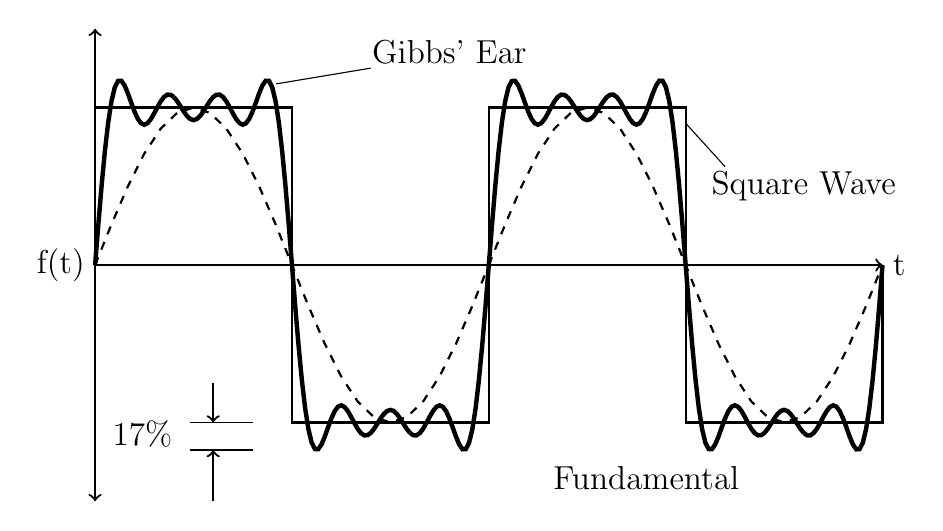
\begin{tikzpicture}

\draw[thick,<->] (0,-3)--(0,3); %yaxis
\draw[thick,->](0,0)--(10,0); %xaxis

%some labels
\node[thick,left,font=\large] at (0,0){f(t)};
\node[thick,right,font=\large] at (10,0){t};
\node[thick,font=\large] at (4.5,2.7){Gibbs' Ear};
\node[thick,font=\large] at (9,1){Square Wave};
\node[thick,font=\large] at (7,-2.7){Fundamental};
\node[thick,font=\large] at (.6,-2.15){17\%};

%some lines
\draw[thick,->] (1.5,-3)--(1.5,-2.35);
\draw[thick,->] (1.5,-1.5)--(1.5,-2);
\draw(1.2,-2)--(2,-2);
\draw(1.2,-2.35)--(2,-2.35);
\draw(3.5,2.5)--(2.3,2.3);
\draw(8,1.25)--(7.5,1.8);

%some functions
\draw[thick,domain=0:5,dashed] plot (\x, {2*sin(\x*72)}); %first order FS
\draw[thick,domain=5:10,dashed] plot (\x, {2*sin(\x*72)}); %first order FS
\draw[thick](0,2)--(2.5,2)--(2.5,-2)--(5,-2)--(5,2)--(7.5,2)--
(7.5,-2)--(10,-2)--(10,0); %square wave

%4th order FS
\draw[ultra thick,domain=0:1] plot (\x, {2*(1.27*sin(\x*1.2566 r)+.42*sin(\x*3.7699 r)+.25*sin(\x*6.2832 r)
+.18*sin(\x*8.7965 r))});
\draw[ultra thick,domain=1:2] plot (\x, {2*(1.27*sin(\x*1.2566 r)+.42*sin(\x*3.7699 r)+.25*sin(\x*6.2832 r)
+.18*sin(\x*8.7965 r))});
\draw[ultra thick,domain=2:3] plot (\x, {2*(1.27*sin(\x*1.2566 r)+.42*sin(\x*3.7699 r)+.25*sin(\x*6.2832 r)
+.18*sin(\x*8.7965 r))});
\draw[ultra thick,domain=3:4] plot (\x, {2*(1.27*sin(\x*1.2566 r)+.42*sin(\x*3.7699 r)+.25*sin(\x*6.2832 r)
+.18*sin(\x*8.7965 r))});
\draw[ultra thick,domain=4:5] plot (\x, {2*(1.27*sin(\x*1.2566 r)+.42*sin(\x*3.7699 r)+.25*sin(\x*6.2832 r)
+.18*sin(\x*8.7965 r))});
\draw[ultra thick,domain=5:6] plot (\x, {2*(1.27*sin(\x*1.2566 r)+.42*sin(\x*3.7699 r)+.25*sin(\x*6.2832 r)
+.18*sin(\x*8.7965 r))});
\draw[ultra thick,domain=6:7] plot (\x, {2*(1.27*sin(\x*1.2566 r)+.42*sin(\x*3.7699 r)+.25*sin(\x*6.2832 r)
+.18*sin(\x*8.7965 r))});
\draw[ultra thick,domain=7:8] plot (\x, {2*(1.27*sin(\x*1.2566 r)+.42*sin(\x*3.7699 r)+.25*sin(\x*6.2832 r)
+.18*sin(\x*8.7965 r))});
\draw[ultra thick,domain=8:9] plot (\x, {2*(1.27*sin(\x*1.2566 r)+.42*sin(\x*3.7699 r)+.25*sin(\x*6.2832 r)
+.18*sin(\x*8.7965 r))});
\draw[ultra thick,domain=9:10] plot (\x, {2*(1.27*sin(\x*1.2566 r)+.42*sin(\x*3.7699 r)+.25*sin(\x*6.2832 r)
+.18*sin(\x*8.7965 r))});
\end{tikzpicture}

\caption{An illustration of Gibbs' phenomenon.}
\label{fig:fs3}
\end{figure}








\newpage
\section{Standard lab equipment}

\begin{figure}[h!]
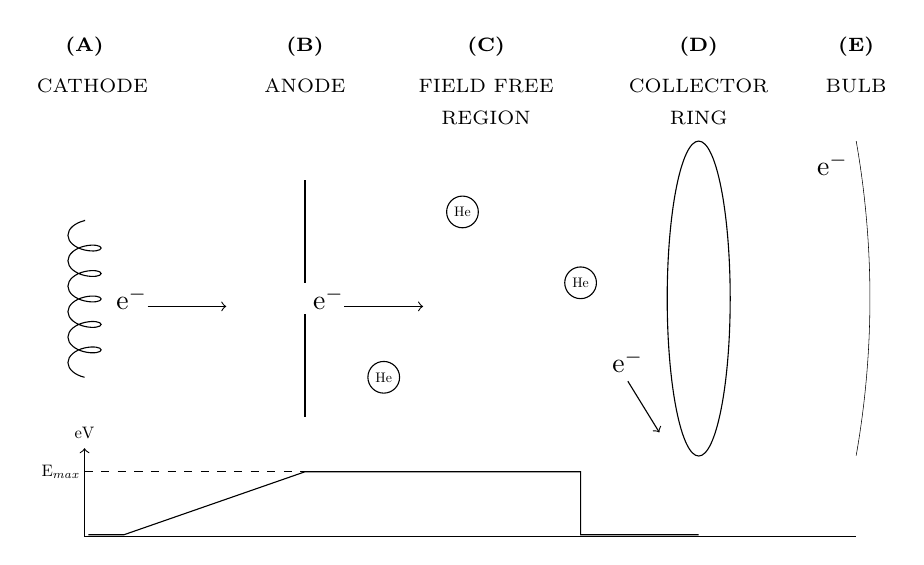
\begin{tikzpicture}

%filament
\draw[decorate, decoration={coil, amplitude=6, segment length=9.2}](.2,3)--(.2,5);
%accelerating cathode
\draw[](3,2.5)--(3,3.8);
\draw[](3,5.5)--(3,4.2);
%electrons
\node[]at(.8,4){e$^-$};
\node[]at(3.3,4){e$^-$};
\node[]at(7.1,3.2){e$^-$};
\node[]at(9.7,5.7){e$^-$};
%helium atoms
\node[draw,circle,scale=.5]at(5,5.1){He};
\node[draw,circle,scale=.5]at(6.5,4.2){He};
\node[draw,circle,scale=.5]at(4,3){He};
\draw[->](1,3.9)--(2,3.9);
\draw[->](3.5,3.9)--(4.5,3.9);
\draw[->](7.1,2.95)--(7.5,2.3);
%collector ring
\draw[](8,4)ellipse(.4 and 2);
%anode
\draw[very thin](10,6)arc(10:-10:11.5);
%energy plot
\draw[](.25,1)--(.7,1)--(3,1.8)--(6.5,1.8)--(6.5,1)--(8,1);
\draw[<-](.2,2.1)--(.2,.98)--(10,.98);
\node[scale=.6]at(.2,2.3){eV};
\draw[dashed](.2,1.8)--(3,1.8);
\node[scale=.6]at(-.1,1.8){E$_{max}$};
%labels
\node[font=\scriptsize]at(.2,7.2){{\bf (A)}};
\node[font=\scriptsize]at(3,7.2){{\bf (B)}};
\node[font=\scriptsize]at(5.3,7.2){{\bf (C)}};
\node[font=\scriptsize]at(8,7.2){{\bf (D)}};
\node[font=\scriptsize]at(10,7.2){{\bf (E)}};
\node[font=\scriptsize]at(10,6.7){BULB};
\node[font=\scriptsize]at(8,6.7){COLLECTOR};
\node[font=\scriptsize]at(8,6.3){RING};
\node[font=\scriptsize]at(5.3,6.7){FIELD FREE};
\node[font=\scriptsize]at(5.3,6.3){REGION};
\node[font=\scriptsize]at(3,6.7){ANODE};
\node[font=\scriptsize]at(.3,6.7){CATHODE};

\end{tikzpicture}
\caption{An illustration depicting the journey of an electron within the Franck-Hertz tube. The energy of colliding electrons is charted along the bottom of the diagram.}
\label{fig:cpTheory}
\end{figure}



\begin{figure}
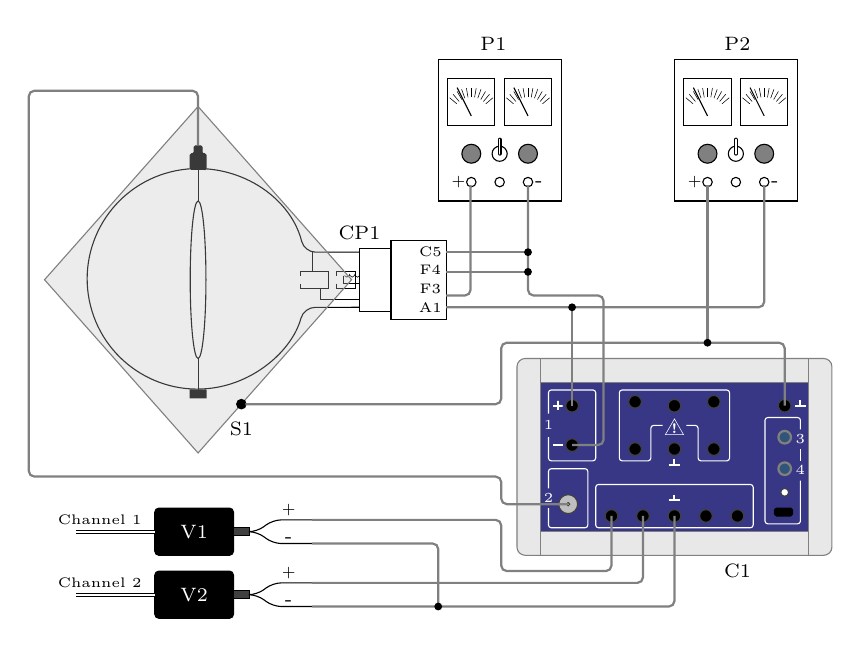
\begin{tikzpicture}
%\draw[ultra thin, lightgray](0,0)rectangle(11,9);

\foreach \x/\y in {5/6.5,8/6.5}{
%power supply
\begin{scope}[shift={(\x,\y)},scale=1.2]
%power supply outline
\draw[](0,0)rectangle(1.3,1.5);
\draw[](.1,.8)rectangle(.6,1.3);
\draw[](.7,.8)rectangle(1.2,1.3);

%power supply indicators
\draw[](.35,.9)--(.2,1.2);
\draw[shift={(.6,0)}](.35,.9)--(.2,1.2);

%power supply right indicator demarcation
\begin{scope}[shift={(.95,.9)}]
\foreach \a in {0,10,...,100}{
\draw[very thin, rotate=40+\a](.2,0)--(.3,0);
}
\end{scope}

%power supply left indicator demarcation
\begin{scope}[shift={(.35,.9)}]
\foreach \a in {0,10,...,100}{
\draw[very thin, rotate=40+\a](.2,0)--(.3,0);
}
\end{scope}

%power supply knobs and power switch
\draw[fill=gray](.35,.5)circle(.1);
\draw[fill=gray](.95,.5)circle(.1);
\draw[](.65,.5)circle(.08);
\draw[fill=white,double,line cap=round](.65,.5)--(.65,.65);

%power supply terminals
\draw[](.35,.2)circle(.05)node[font=\tiny,left=-2]{$_+$};
\draw[](.95,.2)circle(.05)node[font=\scriptsize,right=-1]{-};
\draw[](.65,.2)circle(.05);
\end{scope}
}

\begin{scope}[shift={(5.1,5)},xscale=-1]
%critical potential tube
\draw[](0,0)rectangle(.7,1);
\draw[](.7,.1)rectangle(1.1,.9);
\draw[rounded corners=4](1.1,.85)--(1.8,.85)arc(166:-165:1.4)--(1.1,.15);

%e-gun and accelerator
\draw[very thin](1.1,.45)--(1.3,.45)--(1.3,.55);
\draw[very thin,decorate,decoration={coil, segment length=1.9, amplitude=.5}](1.1,.55)--(1.3,.55);
\draw[very thin](1.4,.45)--(1.4,.39)--(1.15,.39)--(1.15,.61)--(1.4,.61)--(1.4,.55);
\draw[very thin,shift={(.35,0)}](1.5,.45)--(1.5,.39)--(1.15,.39)--(1.15,.61)--(1.5,.61)--(1.5,.55);
\draw[very thin](1.6,.39)--(1.6,.25)--(1.1,.25);
\draw[very thin](1.7,.61)--(1.7,.85);

%collector
\draw[](3.15,.5)ellipse(.1 and 1);
\draw[](3.15,1.5)--(3.15,1.9);
\draw[](3.15,-.5)--(3.15,-.9);
\draw[fill,rounded corners=.5](3.05,1.9)--(3.05,2.1)--(3.1,2.1)--(3.1,2.2)--(3.2,2.2)--(3.2,2.1)--(3.25,2.1)--(3.25,1.9)arc(86:94:1.4);
\draw[fill](3.05,-.9)--(3.05,-1)--(3.25,-1)--(3.25,-.9)arc(-86:-94:1.4);

%shield
\draw[gray,fill=lightgray,fill opacity=.3](1.2,.5)--(3.15,2.7)--(5.1,.5)--(3.15,-1.7)--cycle;
\draw[fill](2.6,-1.08)circle(.06);

%label
\node[font=\tiny]at(.2,.85){C5};
\node[font=\tiny]at(.2,.62){F4};
\node[font=\tiny]at(.2,.38){F3};
\node[font=\tiny]at(.2,.15){A1};
\end{scope}

%controller
\begin{scope}[shift={(6,2)}]
\draw[rounded corners=3, draw=gray, fill={rgb:black,.1;white,1}](0,0)rectangle(4,2.5);
\draw[gray](.3,2.5)--(.3,0);
\draw[gray](3.7,2.5)--(3.7,0);
\draw[draw=gray,fill={rgb:red,1;green,1;blue,2.4;black,.2}](.3,.3)rectangle(3.7,2.2);

%terminals
\foreach \x/\y in {.7/1.4,.7/1.9,1.2/.5,1.6/.5,2/.5,2.4/.5,2.8/.5,1.5/1.35,2/1.35,2.5/1.35,1.5/1.95,2/1.9,2.5/1.95,3.4/1.9}{
\draw[draw=darkgray,fill=black](\x,\y)circle(.08);
}
\draw[draw=gray,fill={rgb:red,.4;green,.7;blue,1},thick](3.4,1.1)circle(.08);
\draw[draw=gray,fill={rgb:red,.4;green,.7;blue,1},thick](3.4,1.5)circle(.08);
\draw[draw=darkgray,fill=white](3.4,.8)circle(.05);
\draw[draw=darkgray,fill=lightgray](.65,.65)circle(.12);
\draw[draw=darkgray,fill=white](.65,.65)circle(.02);

%white lines
\draw[white,rounded corners=1](1,.35)--(1,.9)--(3,.9)--(3,.35)--cycle;
\draw[white,rounded corners=1](.4,.6)--(.4,.35)--(.9,.35)--(.9,1.1)--(.4,1.1)--(.4,.85);
\node[white,font=\tiny]at(.4,.73){2};
\draw[white,rounded corners=1](.4,1.5)--(.4,1.2)--(1,1.2)--(1,2.1)--(.4,2.1)--(.4,1.8);
\node[white,font=\tiny]at(.4,1.65){1};
\draw[white,rounded corners=1](1.85,1.65)--(1.7,1.65)--(1.7,1.2)--(1.3,1.2)--(1.3,2.1)--(2.7,2.1)--(2.7,1.2)--(2.3,1.2)--
(2.3,1.65)--(2.15,1.65);
\node[very thin,regular polygon, regular polygon sides=3,scale=.4,draw=white]at(2,1.6){};
\node[white,font=\tiny]at(2,1.61){{\bf !}};
\draw[white,rounded corners=1](3.6,.95)--(3.6,.4)--(3.15,.4)--(3.15,1.75)--(3.6,1.75)--(3.6,1.6);
\draw[white,rounded corners=1](3.6,1.2)--(3.6,1.35);
\node[white,font=\tiny]at(3.6,1.48){3};
\node[white,font=\tiny]at(3.6,1.08){4};
\draw[fill, rounded corners=.7](3.27,.5)rectangle(3.5,.6);

%ground labels
\foreach \x/\y in {2/1.15,2/.7,3.6/1.9}{
\begin{scope}[shift={(\x,\y)}]
\draw[white,line width=.7](-.07,0)--(.07,0)--(0,0)--(0,.07);
\end{scope}
}

%positive/negative labels
\draw[white,line width=.7,shift={(.52,1.9)}](-.06,0)--(.06,0)--(0,0)--(0,.06)--(0,-.06);
\draw[white,line width=.7](.46,1.4)--(.58,1.4);
\end{scope}

%vernier voltage probes
\foreach \x/\y in {1.4/2,1.4/1.2}{
\begin{scope}[shift={(\x,\y)}]
\draw[fill,rounded corners=1.5](0,0)rectangle(1,.6);
\draw[fill=darkgray](1,.25)rectangle(1.2,.35);
\draw[rounded corners=3](1.2,.3)--(1.3,.3)--(1.5,.45)--(1.7,.45)node[above=-2,font=\tiny]{+}--(2,.45);
\draw[rounded corners=3](1.2,.3)--(1.3,.3)--(1.5,.15)--(1.7,.15)node[above=-3,font=\scriptsize]{-}--(2,.15);
\draw[double](0,.3)--(-1,.3);
\end{scope}
}
\node[font=\tiny]at(.7,2.45){Channel 1};
\node[font=\tiny]at(.7,1.65){Channel 2};

%wires
\draw[rounded corners=2,thick,gray](2.55,3.92)--(5.8,3.92)--(5.8,4.7)--(9.4,4.7)--(9.4,3.9);
\draw[rounded corners=2,thick,gray](1.95,7.21)--(1.95,7.9)--(-.2,7.9)--(-.2,3)--(5.8,3)--(5.8,2.65)--(6.65,2.65);
\draw[rounded corners=2,thick,gray](8.42,6.7)--(8.42,4.7)node[circle,fill=black,scale=.3]{};
\draw[rounded corners=2,thick,gray](9.14,6.7)--(9.14,5.15)--(5.1,5.15);
\draw[rounded corners=2,thick,gray](6.7,3.9)--(6.7,5.15)node[circle,fill=black,scale=.3]{};
\draw[rounded corners=2,thick,gray](6.14,6.7)--(6.14,5.3)--(7.1,5.3)--(7.1,3.4)--(6.7,3.4);
\draw[rounded corners=2,thick,gray](5.41,6.7)--(5.41,5.3)--(5.1,5.3);
\draw[rounded corners=2,thick,gray](5.1,5.6)--(6.14,5.6)node[circle,fill=black,scale=.3]{};
\draw[rounded corners=2,thick,gray](5.1,5.85)--(6.14,5.85)node[circle,fill=black,scale=.3]{};
\draw[rounded corners=2,thick,gray](3.4,2.45)--(5.8,2.45)--(5.8,1.8)--(7.2,1.8)--(7.2,2.5);
\draw[rounded corners=2,thick,gray](3.4,1.65)--(7.6,1.65)--(7.6,2.5);
\draw[rounded corners=2,thick,gray](3.4,1.35)--(8,1.35)--(8,2.5);
\draw[rounded corners=2,thick,gray](3.4,2.15)--(5,2.15)--(5,1.35)node[fill=black,circle,scale=.3]{};

%labels
\node[font=\scriptsize]at(5.7,8.5){P1};
\node[font=\scriptsize]at(8.8,8.5){P2};
\node[font=\scriptsize,white]at(1.9,2.3){V1};
\node[font=\scriptsize,white]at(1.9,1.5){V2};
\node[font=\scriptsize]at(8.8,1.8){C1};
\node[font=\scriptsize]at(2.5,3.6){S1};
\node[font=\scriptsize]at(4,6.1){CP1};

\end{tikzpicture}
\caption{Wiring diagram for the experiment. Shown in the diagram are the cathode power supply, P1, the anode bias power supply, P2, the Vernier voltage probe recording the ramping voltage, V1, the Vernier voltage probe recording the collector ring current, V2, the critical potential tube controller, C1, the critical potential tube, CP1, and the shielding meant to isolate the tube from EM interference, S1.}
\label{fig:cpSetup}
\end{figure}


\begin{figure}%fig4
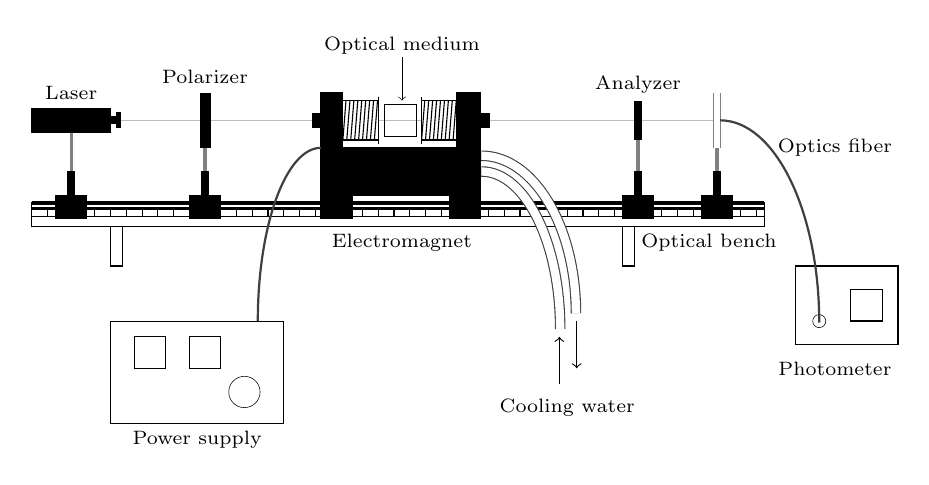
\begin{tikzpicture}
%\draw[very thin](0,0)rectangle(11,6);
%optical axis
\draw[ultra thin,lightgray](0,4.85)--(8.7,4.85);
%optical bench
\draw[](0,3.5)rectangle(9.3,3.8);
\draw[very thick](0,3.8)--(9.3,3.8);
\draw[very thick](0,3.73)--(9.3,3.73);
\draw[thin](0,3.63)--(9.3,3.63);
\foreach \x in {0,.2,...,9.2}{
\draw[thin](0+\x,3.63)--(0+\x,3.73);
}
\draw[](1,3)rectangle(1.15,3.5);
\draw[](7.5,3)rectangle(7.65,3.5);
%bench clamps
\foreach \x in {.3,2,3.67,5.3,7.5,8.5}{
\draw[fill](0+\x,3.6)rectangle(.4+\x,3.9);
\draw[line width=3](.2+\x,3.8)--(.2+\x,4.2);
\draw[very thick,gray](.2+\x,4.2)--(.2+\x,4.7);
}
%electromagnet
\draw[fill](3.67,3.9)--(3.67,5.2)--(3.95,5.2)--(3.95,4.5)--(5.4,4.5)
--(5.4,5.2)--(5.7,5.2)--(5.7,3.9)--cycle;
\node[shape=rectangle,scale=.8,fill]at(3.65,4.85){};
\node[shape=rectangle,scale=.8,fill]at(5.72,4.85){};
\begin{scope}
\draw[fill=white](3.95,4.6)rectangle(4.4,5.1);
\foreach \x in {0,.05,...,.44}{
\draw[](3.95+\x,4.6)--(3.99+\x,5.1);
}
\draw[](3.95,4.55)--(3.95,5.15);
\draw[](4.4,4.55)--(4.4,5.15);
\end{scope}
\begin{scope}[shift={(1,0)}]
\draw[fill=white](3.95,4.6)rectangle(4.4,5.1);
\foreach \x in {0,.05,...,.44}{
\draw[](3.95+\x,4.6)--(3.99+\x,5.1);
}
\draw[](3.95,4.55)--(3.95,5.15);
\draw[](4.4,4.55)--(4.4,5.15);
\end{scope}
\draw[very thin](4.48,4.65)rectangle(4.88,5.05);
%"frickin' laser beams"
\draw[fill](0,4.7)rectangle(1,5.);
\draw[line width=3](0,4.85)--(1.1,4.85);
\draw[line width=2](1.1,4.75)--(1.1,4.95);
%polarizer
\draw[line width=4](2.2,4.5)--(2.2,5.2);
%analyzer
\draw[line width=3](7.7,4.6)--(7.7,5.1);
%screen with optical fiber
\draw[double distance=2,draw=gray](8.7,4.5)--(8.7,5.2);
%power supply
\draw[](1,1)rectangle(3.2,2.3);
\node[thin,shape=rectangle,scale=1.7,draw]at(1.5,1.9){};
\node[thin,shape=rectangle,scale=1.7,draw]at(2.2,1.9){};
\node[very thin,shape=circle,scale=1.2,draw]at(2.7,1.4){};
\draw[thick,darkgray](3.67,4.5)arc(90:180:.8 and 2.2);
%photometer
\draw[](11,3)rectangle(9.7,2);
\node[thin,shape=rectangle,scale=1.7,draw]at(10.6,2.5){};
\node[very thin,shape=circle,scale=.5,draw]at(10,2.3){};
\draw[thick,darkgray](8.74,4.85)arc(90:0:1.26 and 2.57);
%cooling lines
\draw[double distance=3,darkgray](5.71,4.2)arc(90:0:1 and 2);
\draw[double distance=3,darkgray](5.71,4.4)arc(90:0:1.2 and 2.);
\draw[<-](6.7,2.1)--(6.7,1.5);
\draw[->](6.92,2.3)--(6.92,1.7);
%labels
\node[font=\scriptsize]at(.5,5.2){Laser};
\node[font=\scriptsize]at(2.2,5.4){Polarizer};
\node[font=\scriptsize]at(4.7,5.8){Optical medium};
\draw[->,very thin](4.7,5.65)--(4.7,5.1);
\node[font=\scriptsize]at(7.7,5.3){Analyzer};
\node[font=\scriptsize]at(10.2,4.5){Optics fiber};
\node[font=\scriptsize]at(8.6,3.3){Optical bench};
\node[font=\scriptsize]at(4.7,3.3){Electromagnet};
\node[font=\scriptsize]at(2.1,.8){Power supply};
\node[font=\scriptsize]at(6.8,1.2){Cooling water};
\node[font=\scriptsize]at(10.2,1.7){Photometer};

\end{tikzpicture}
\caption{Experimental Setup}
\label{fig:feExperimentalSetup}
\end{figure}





\begin{figure}
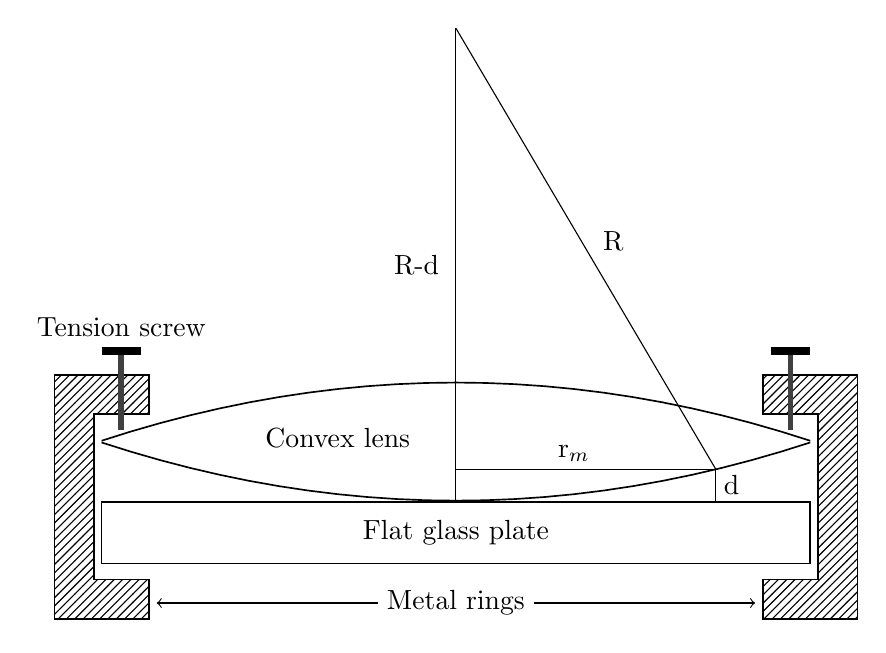
\begin{tikzpicture}[semithick]
%parabolic convex lens
\draw[domain=1:10] plot (\x, {(0.0365)*pow(\x-5.5,2)+2});
\draw[domain=1:10] plot (\x, {(-0.0365)*pow(\x-5.5,2)+3.5});
%glass plate
\draw[](1,1.2)rectangle(10,1.98);
%metal rings
\draw[pattern=north east lines](.4,.5)--(.4,3.6)--(1.6,3.6)--(1.6,3.1)--(.9,3.1)--(.9,1)--
(1.6,1)--(1.6,.5)--cycle;
\draw[pattern=north east lines,rotate=180,shift={(-11,-4.1)}](.4,.5)--(.4,3.6)--(1.6,3.6)--(1.6,3.1)--(.9,3.1)--(.9,1)--
(1.6,1)--(1.6,.5)--cycle;
%tension screws
\draw[line width=2pt,draw=darkgray](1.25,3.9)--(1.25,2.9);
\draw[line width=2pt,draw=darkgray](9.75,3.9)--(9.75,2.9);
\draw[line width=3pt](1,3.9)--(1.5,3.9);
\draw[line width=3pt](9.5,3.9)--(10,3.9);
%demarcation lines
\begin{scope}[thin,font=\normalsize]
\draw[](5.5,8)--(5.5,2);
\draw[](5.5,2.4)--(8.8,2.4);
\draw[](5.5,8)--(8.8,2.4);
\draw[](8.8,2)--(8.8,2.4);
%labels
\node[]at(7.5,5.3){R};
\node[]at(5,5){R-d};
\node[]at(9,2.2){d};
\node[]at(7,2.6){r$_m$};
\node[]at(4,2.8){Convex lens};
\node[]at(1.25,4.2){Tension screw};
\node[]at(5.5,1.6){Flat glass plate};
\draw[<->](1.7,.7)--(9.3,.7);
\node[fill=white]at(5.5,.7){Metal rings};
\end{scope}
\end{tikzpicture}
\caption{Experimental setup for the investigation of Newton rings.}
\label{fig:fb4}
\end{figure}





\begin{figure}
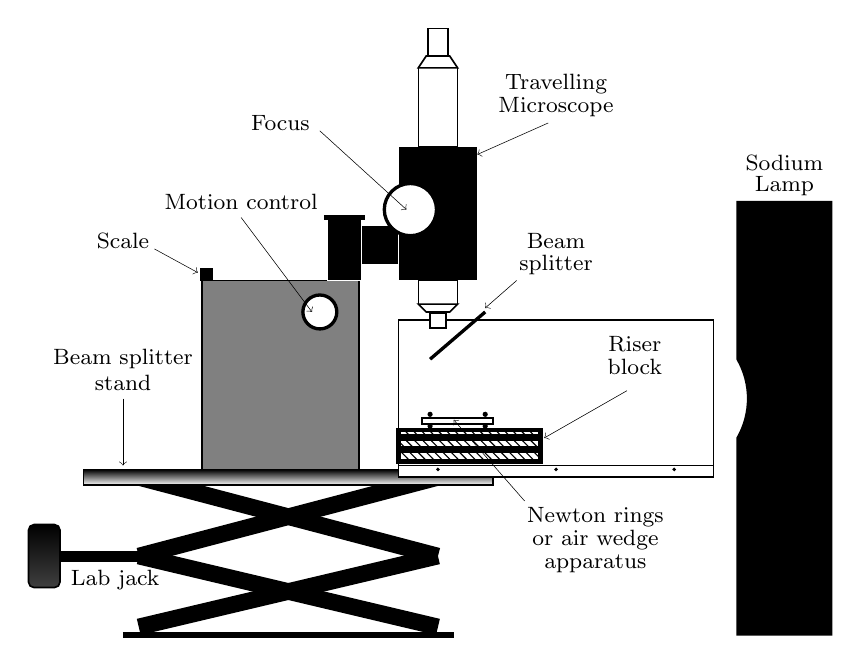
\begin{tikzpicture}[semithick]
%sodium lamp
\draw[fill](9.8,0)--(9.8,2.5)arc(-30:30:1)--(9.8,5.5)--(11,5.5)--(11,0)--cycle;
%laboratory Jack
\draw[line width=2pt](2,0)--(6.2,0);
\draw[line width=6pt](2.2,.1)--(6,1);
\draw[line width=6pt](2.2,2)--(6,1);
\draw[line width=6pt](2.2,1)--(6,.1);
\draw[line width=6pt](6,2)--(2.2,1);
\draw[shade,top color=black](1.5,1.9)rectangle(6.7,2.1);
\draw[rounded corners=2,shade,top color=black,bottom color=darkgray](.8,.6)rectangle(1.2,1.4);
\draw[line width=4](1.2,1)--(2.2,1);
%platform
\draw[fill=white](9.5,2)rectangle(5.5,4);
\draw[](5.5,2.15)--(9.5,2.15);
\node[circle,scale=.15,fill]at(6,2.1){};
\node[circle,scale=.15,fill]at(7.5,2.1){};
\node[circle,scale=.15,fill]at(9,2.1){};
%microscope
\draw[draw,fill=gray](3,2.1)rectangle(5,4.5);
\node[circle,scale=1.3,fill=white,draw,very thick]at(4.5,4.1){};
\node[rectangle,scale=.7,fill]at(3.06,4.58){};
\draw[fill,draw=white,thin](5,4.7)rectangle(5.5,5.2);
\draw[fill,draw=white,thin](4.6,4.5)rectangle(5.03,5.3);
\draw[line width=2](4.55,5.3)--(5.07,5.3);
\draw[fill,draw=white,thin](5.5,4.5)rectangle(6.5,6.2);
\draw[fill=white,draw=black,thin](5.75,6.2)rectangle(6.25,7.2);
\draw[](5.75,7.2)--(5.85,7.35)--(6.15,7.35)--(6.25,7.2)--cycle;
\draw[](5.87,7.35)rectangle(6.13,7.7);
\node[circle,scale=2,fill=white,draw,very thick]at(5.65,5.4){};
\draw[fill=white,draw=black,thin](5.75,4.5)rectangle(6.25,4.2);
\draw[](5.75,4.2)--(5.85,4.1)--(6.15,4.1)--(6.25,4.2)--cycle;
\draw[fill=white](5.9,3.9)rectangle(6.1,4.08);
%beam splitter
\draw[very thick](6.6,4.1)--(5.9,3.5);
%riser block
\draw[ultra thick,pattern=north west lines](5.5,2.2)rectangle(7.3,2.6);
\draw[line width=2.5](5.5,2.5)--(7.3,2.5);
\draw[line width=2.5](5.5,2.35)--(7.3,2.35);
%newton rings apparatus
\draw[thick](5.8,2.75)rectangle(6.7,2.68);
\node[circle,scale=.2,fill]at(5.9,2.8){};
\node[circle,scale=.2,fill]at(6.6,2.8){};
\node[circle,scale=.2,fill]at(5.9,2.65){};
\node[circle,scale=.2,fill]at(6.6,2.65){};
%labels
\begin{scope}[very thin,font=\footnotesize,->]
\node at(1.9,.7){Lab jack};
\node at(2,5){Scale};
\draw(2.4,4.9)--(2.95,4.6);
\node at(2,3.5){Beam splitter};
\node at(2,3.2){stand};
\draw(2,3)--(2,2.15);
\node at(3.5,5.5){Motion control};
\draw(3.5,5.3)--(4.4,4.1);
\node at(4,6.5){Focus};
\draw(4.5,6.4)--(5.6,5.4);
\node at(7.5,7){Travelling};
\node at(7.5,6.7){Microscope};
\draw(7.4,6.5)--(6.5,6.1);
\node at(7.5,5){Beam};
\node at(7.5,4.7){splitter};
\draw(7,4.5)--(6.6,4.15);
\node at(8.5,3.7){Riser};
\node at(8.5,3.4){block};
\draw(8.4,3.1)--(7.35,2.5);
\node at(8,1.5){Newton rings};
\node at(8,1.2){or air wedge};
\node at(8,.9){apparatus};
\draw(7.1,1.7)--(6.2,2.73);
\node at(10.4,6){Sodium};
\node at(10.4,5.7){Lamp};
\end{scope}
\end{tikzpicture}
\caption{Experimental setup used to measure the spacing between Fizeau bands.}
\label{fig:fb6}
\end{figure}



\begin{figure}
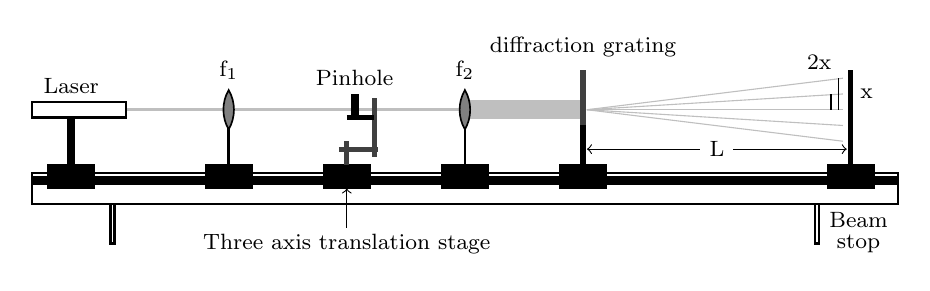
\begin{tikzpicture}
%\draw[very thin](0,0)rectangle(11,7);
%optical bench
\draw[thick](0,.5)rectangle(11,.9);
\draw[thick](1,0)rectangle(1.05,.5);
\draw[thick](9.95,0)rectangle(10,.5);
\draw[line width=3](0,.8)--(11,.8);
%beam
\draw[line width=1,draw=lightgray](1.2,1.7)--(5.5,1.7);
\draw[line width=7,draw=lightgray](7,1.7)--(5.5,1.7);
%grating
\begin{scope}[shift={(6.5,0)}]
\draw[fill](.2,.7)rectangle(.8,1);
\draw[line width=2,draw=darkgray](.5,.9)--(.5,2.2);
\draw[line width=2](.5,.9)--(.5,1.5);
\end{scope}
%laser
\draw[fill](.2,.7)rectangle(.8,1);
\draw[line width=3](.5,.9)--(.5,1.6);
\draw[thick](0,1.6)rectangle(1.2,1.8);
%f1
\begin{scope}[shift={(2,0)}]
\draw[fill](.2,.7)rectangle(.8,1);
\draw[line width=1](.5,.9)--(.5,1.6);
\draw[line width=.6,fill=gray](.5,1.45)arc(-30:30:.5)arc(-30:30:-.5);
\end{scope}
%f2
\begin{scope}[shift={(5,0)}]
\draw[fill](.2,.7)rectangle(.8,1);
\draw[line width=1](.5,.9)--(.5,1.6);
\draw[line width=.6,fill=gray](.5,1.45)arc(-30:30:.5)arc(-30:30:-.5);
\end{scope}
%diffracted beam
\foreach \y in {0,.2,.4,.6,.8}{
\draw[draw=lightgray](7.05,1.7)--(10.3,1.3+\y);
}
%pinhole
\begin{scope}[shift={(3.5,0)}]
\draw[fill](.2,.7)rectangle(.8,1);
\draw[line width=1.8,draw=darkgray](.5,1)--(.5,1.3);
\draw[line width=1.8,draw=darkgray](.4,1.2)--(.9,1.2);
\draw[line width=1.8,draw=darkgray](.85,1.1)--(.85,1.85);
\draw[line width=1.8](.5,1.6)--(.85,1.6);
\draw[line width=3](.6,1.6)--(.6,1.9);
\end{scope}
%beam stop
\begin{scope}[shift={(9.9,0)}]
\draw[fill](.2,.7)rectangle(.8,1);
\draw[line width=2](.5,.9)--(.5,2.2);
\end{scope}
%demarcation lines
\draw[thin,<->](7.05,1.2)--(10.35,1.2);
\draw[thin](10.25,1.7)--(10.25,2.1);
\draw[thin](10.15,1.7)--(10.15,1.9);
%labels
\node[font=\footnotesize]at(.5,2){Laser};
\node[font=\footnotesize]at(4.1,2.1){Pinhole};
\node[font=\footnotesize]at(4,0){Three axis translation stage};
\draw[->,thin](4,.2)--(4,.7);
\node[font=\footnotesize]at(2.5,2.2){f$_1$};
\node[font=\footnotesize]at(5.5,2.2){f$_2$};
\node[font=\footnotesize]at(7,2.5){diffraction grating};
\node[font=\footnotesize]at(10.5,.3){Beam};
\node[font=\footnotesize]at(10.5,0){stop};
\node[font=\footnotesize]at(10.6,1.9){x};
\node[font=\footnotesize]at(10,2.3){2x};
\node[font=\footnotesize,fill=white]at(8.7,1.2){L};
\end{tikzpicture}
\caption{ }
\label{fig:lb14}
\end{figure}




\begin{figure}
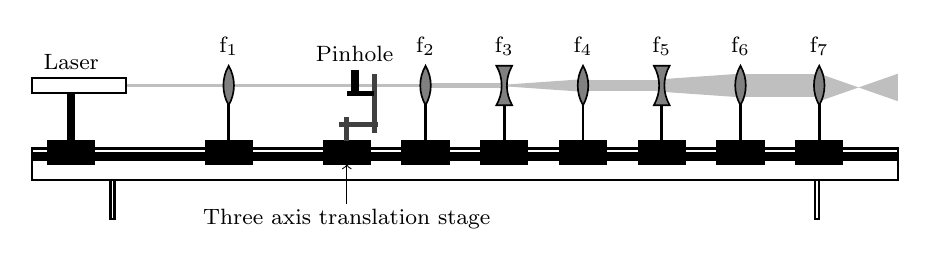
\begin{tikzpicture}
%\draw[very thin](0,0)rectangle(11,7);
%optical bench
\draw[thick](0,.5)rectangle(11,.9);
\draw[thick](1,0)rectangle(1.05,.5);
\draw[thick](9.95,0)rectangle(10,.5);
\draw[line width=3](0,.8)--(11,.8);
%beam
\draw[line width=1,draw=lightgray](1.2,1.7)--(5,1.7);
\draw[line width=2,draw=lightgray](6,1.7)--(5,1.7);
\draw[draw=none,fill=lightgray](6,1.71)--(7,1.78)--(7,1.62)--(6,1.69);
\draw[line width=4,draw=lightgray](7,1.7)--(8,1.7);
\draw[draw=none,fill=lightgray](8,1.78)--(9,1.85)--(9,1.55)--(8,1.62);
\draw[line width=8,draw=lightgray](9,1.7)--(10,1.7);
\draw[fill=lightgray,draw=none](10,1.85)--(11,1.5)--(11,1.85)--(10,1.5);
%laser
\draw[fill](.2,.7)rectangle(.8,1);
\draw[line width=3](.5,.9)--(.5,1.6);
\draw[thick](0,1.6)rectangle(1.2,1.8);
%f1
\begin{scope}[shift={(2,0)}]
\draw[fill](.2,.7)rectangle(.8,1);
\draw[line width=1](.5,.9)--(.5,1.6);
\draw[line width=.6,fill=gray](.5,1.45)arc(-30:30:.5)arc(-30:30:-.5);
\end{scope}
%f2
\begin{scope}[shift={(4.5,0)}]
\draw[fill](.2,.7)rectangle(.8,1);
\draw[line width=1](.5,.9)--(.5,1.6);
\draw[line width=.6,fill=gray](.5,1.45)arc(-30:30:.5)arc(-30:30:-.5);
\end{scope}
%f3
\begin{scope}[shift={(5.5,0)}]
\draw[fill](.2,.7)rectangle(.8,1);
\draw[line width=1](.5,.9)--(.5,1.6);
\draw[line width=.6,fill=gray](.4,1.45)arc(-30:30:.5)--(.6,1.95)arc(-30:30:-.5)--cycle;
\end{scope}
%f5
\begin{scope}[shift={(7.5,0)}]
\draw[fill](.2,.7)rectangle(.8,1);
\draw[line width=1](.5,.9)--(.5,1.6);
\draw[line width=.6,fill=gray](.4,1.45)arc(-30:30:.5)--(.6,1.95)arc(-30:30:-.5)--cycle;
\end{scope}
%f4
\begin{scope}[shift={(6.5,0)}]
\draw[fill](.2,.7)rectangle(.8,1);
\draw[line width=1](.5,.9)--(.5,1.6);
\draw[line width=.6,fill=gray](.5,1.45)arc(-30:30:.5)arc(-30:30:-.5);
\end{scope}
%f6
\begin{scope}[shift={(8.5,0)}]
\draw[fill](.2,.7)rectangle(.8,1);
\draw[line width=1](.5,.9)--(.5,1.6);
\draw[line width=.6,fill=gray](.5,1.45)arc(-30:30:.5)arc(-30:30:-.5);
\end{scope}
%f7
\begin{scope}[shift={(9.5,0)}]
\draw[fill](.2,.7)rectangle(.8,1);
\draw[line width=1](.5,.9)--(.5,1.6);
\draw[line width=.6,fill=gray](.5,1.45)arc(-30:30:.5)arc(-30:30:-.5);
\end{scope}
%pinhole
\begin{scope}[shift={(3.5,0)}]
\draw[fill](.2,.7)rectangle(.8,1);
\draw[line width=1.8,draw=darkgray](.5,1)--(.5,1.3);
\draw[line width=1.8,draw=darkgray](.4,1.2)--(.9,1.2);
\draw[line width=1.8,draw=darkgray](.85,1.1)--(.85,1.85);
\draw[line width=1.8](.5,1.6)--(.85,1.6);
\draw[line width=3](.6,1.6)--(.6,1.9);
\end{scope}
%labels
\node[font=\footnotesize]at(.5,2){Laser};
\node[font=\footnotesize]at(4.1,2.1){Pinhole};
\node[font=\footnotesize]at(4,0){Three axis translation stage};
\draw[->,thin](4,.2)--(4,.7);
\node[font=\footnotesize]at(2.5,2.2){f$_1$};
\node[font=\footnotesize]at(5,2.2){f$_2$};
\node[font=\footnotesize]at(6,2.2){f$_3$};
\node[font=\footnotesize]at(7,2.2){f$_4$};
\node[font=\footnotesize]at(8,2.2){f$_5$};
\node[font=\footnotesize]at(9,2.2){f$_6$};
\node[font=\footnotesize]at(10,2.2){f$_7$};
\end{tikzpicture}
\caption{"Laser beams"}
\label{fig:lb18}
\end{figure}




\begin{figure}
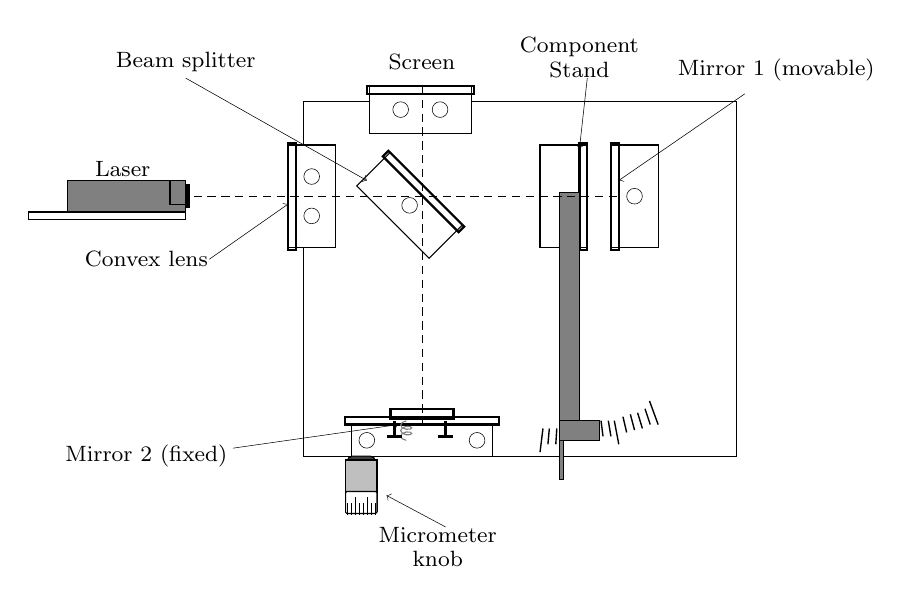
\begin{tikzpicture}
%\draw[very thin](0,0)rectangle(11,8);
%feet
%\node[circle,scale=2,fill]at(3.7,2.5){};
%\node[circle,scale=2,fill]at(9.8,4.8){};
%\node[circle,scale=2,fill]at(9.8,.7){};

%table
\draw[fill=white](9,.5)rectangle(3.5,5);

%laser
\draw[](0,3.5)rectangle(2,3.6);
\draw[fill=gray](.5,3.6)rectangle(2,4);
\draw[very thick](2.03,3.65)--(2.03,3.95);
\draw[](1.8,4)--(1.8,3.7)--(2,3.7);

%Lens and holder
\begin{scope}[rotate=90,shift={(3.15,-3.9)}]
\draw[fill=white](0,0)rectangle(1.3,.6);
\draw[thick](-.03,.6)rectangle(1.33,.5);
\node[circle,very thin,scale=.6,draw]at(.9,.3){};
\node[circle,very thin,scale=.6,draw]at(.4,.3){};
%\draw[line width=2,gray](3.5,3)--(3,3);
\end{scope}

%Screen
\begin{scope}[rotate=0,shift={(4.33,4.6)}]
\draw[fill=white](0,0)rectangle(1.3,.6);
\draw[thick](-.03,.6)rectangle(1.33,.5);
\node[circle,very thin,scale=.6,draw]at(.9,.3){};
\node[circle,very thin,scale=.6,draw]at(.4,.3){};
%\draw[line width=2,gray](3.5,3)--(3,3);
\end{scope}


%beam splitter
\begin{scope}[rotate=-45,shift={(0.17,5.73)}]
\draw[](0,0)rectangle(1.3,.6);
\draw[thick](-.03,.6)rectangle(1.33,.5);
\node[circle,very thin,scale=.6,draw]at(.65,.3){};
\end{scope}

%mirror 1
\begin{scope}[rotate=90,shift={(3.15,-8)}]
\draw[](0,0)rectangle(1.3,.6);
\draw[thick](-.03,.6)rectangle(1.33,.5);
\node[circle,very thin,scale=.6,draw]at(.65,.3){};
\end{scope}

%Mirror 2 (movable)
\begin{scope}[rotate=0,shift={(4.1,0.5)}]
\draw[fill=white](0,0)rectangle(1.8,.4);
\draw[thick](-.08,.4)rectangle(1.88,.5);
\draw[thick](.5,.47)rectangle(1.3,.6);
\node[circle,very thin,scale=.6,draw]at(1.6,.2){};
\node[circle,very thin,scale=.6,draw]at(.2,.2){};
\end{scope}
\draw[decorate,decoration={coil,segment length=2,amplitude=2},draw=gray](4.8,.7)--(4.8,.95);

\draw[line width=1.2](4.65,.75)--(4.65,.95);
\draw[line width=1.2](5.3,.75)--(5.3,.95);
\draw[line width=1.2](4.55,.75)--(4.75,.75);
\draw[line width=1.2](5.2,.75)--(5.4,.75);

\begin{scope}[rotate=90, shift={(-10.25,-6)}]
\draw[fill=darkgray,rounded corners=2](10.5,1.59)rectangle(10.75,1.95);
\draw[fill=lightgray](10.05,1.57)rectangle(10.7,1.97);
\draw[fill=white,rounded corners=.5](10.02,1.57)rectangle(10.3,1.97);
\foreach \y in {0,.05,...,.4}{
\draw[ultra thin](10,1.6+\y)--(10.15,1.6+\y);
}
\foreach \y in {0,.15,...,.2}{
\draw[very thin](10,1.7+\y)--(10.23,1.7+\y);
}
\end{scope}


%stand for glass or air cell
\begin{scope}[rotate=-90,shift={(-4.45,6.5)}]
\draw[](0,0)rectangle(1.3,.6);
\draw[thick](-.03,.6)rectangle(1.33,.5);
\draw[fill=gray](0.6,0.25)rectangle(3.5,0.5);
\draw[fill=gray](3.5,0.25)rectangle(3.75,0.75);
\draw[fill=gray](3.75,0.25)rectangle(4.25,0.30);
\end{scope}

%angle scale

\draw[line width=0.5](6.5,0.55)--(6.537,0.85);
\draw[line width=0.5](6.6,0.65)--(6.618,0.85);
\draw[line width=0.5](6.7,0.65)--(6.713,0.85);

\draw[line width=0.5](7.5,0.65)--(7.443,0.95);
\draw[line width=0.5](7.4,0.75)--(7.367,0.95);
\draw[line width=0.5](7.3,0.75)--(7.274,0.95);

\draw[line width=0.5](8,0.9)--(7.89,1.2);

\draw[line width=0.5](7.6,0.8)--(7.553,1.);
\draw[line width=0.5](7.7,0.83)--(7.647,1.03);
\draw[line width=0.5](7.8,0.85)--(7.739,1.05);
\draw[line width=0.5](7.9,0.90)--(7.8333,1.1);

%optical axes
\draw[very thin,densely dashed](2.1,3.8)--(7.5,3.8);
\draw[very thin,densely dashed](5,5.2)--(5,.9);

%labels
\node[font=\footnotesize]at(1.2,4.15){Laser};
\node[font=\footnotesize]at(1.5,.5){Mirror 2 (fixed)};
\draw[very thin,->](2.6,.6)--(4.7,.9);
\node[font=\footnotesize]at(2,5.5){Beam splitter};
\draw[very thin,->](2,5.3)--(4.3,4);

\node[font=\footnotesize]at(9.5,5.4){Mirror 1 (movable)};
\draw[very thin,->](9.1,5.1)--(7.5,4);

\node[font=\footnotesize]at(5,5.5){Screen};

\node[font=\footnotesize]at(5.2,-0.5){Micrometer};
\node[font=\footnotesize]at(5.2,-.8){knob};
\draw[very thin,->](5.3,-0.4)--(4.55,0);

\node[font=\footnotesize]at(1.5,3){Convex lens};
\draw[very thin,->](2.3,3)--(3.3,3.7);

\node[font=\footnotesize]at(7,5.7){Component};
\node[font=\footnotesize]at(7,5.4){Stand};
\draw[very thin,->](7.1,5.3)--(7,4.4);

\end{tikzpicture}
\caption{A diagram of the interferometer used in this experiment.}
\label{fig:mi1}
\end{figure}








\newpage
\section{Circular Shapes}


\begin{figure}
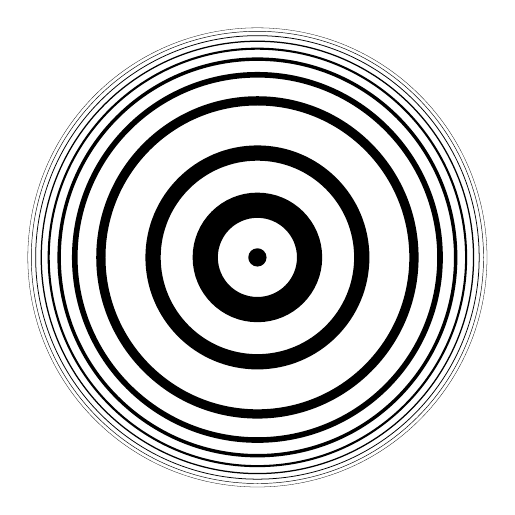
\begin{tikzpicture}[semithick]
\node[fill,circle,scale=.7]at(0,0){};
\foreach \s in {1,2,...,10}{
\node[line width=(15*exp(-\s*.5)),circle,scale=20-24/(\s),draw]at(0,0){};
}
\end{tikzpicture}
\caption{An illustration of Newton rings.}
\label{fig:fb3}
\end{figure}






\newpage
\section{Isometric diagrams}



\begin{figure}%fig1
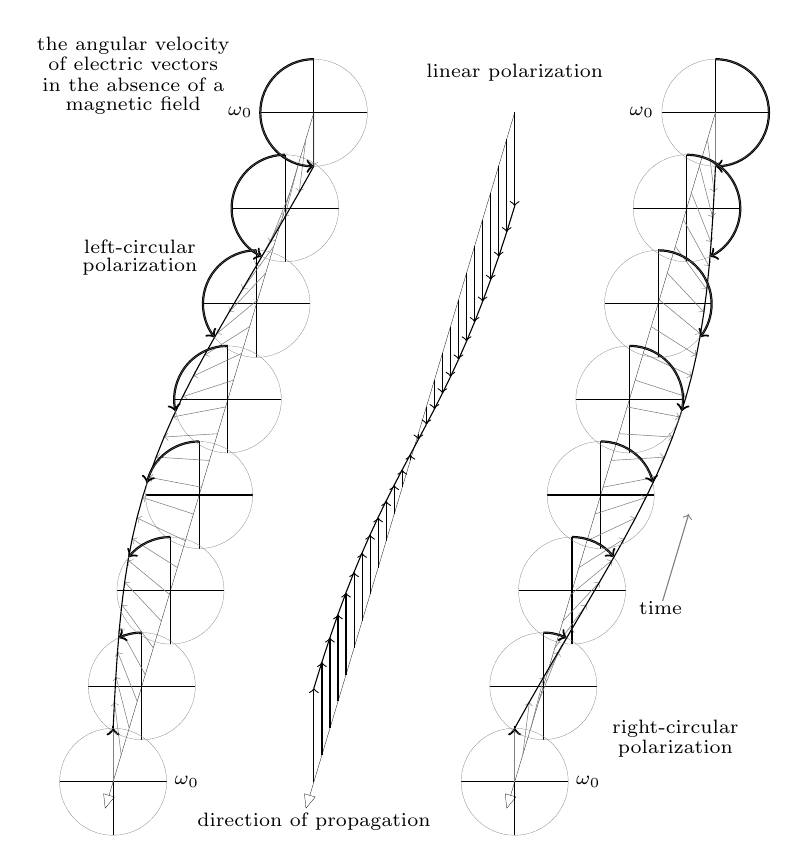
\begin{tikzpicture}[x={(1cm,0cm)}, y={(0cm,1cm)}, z={(.3cm,1cm)}, scale=1.7]
\coordinate (O) at (0, 0, 0);
%linear polarized
\foreach \x in {0,-1.5,1.5}{
\draw[ultra thin,open triangle 45-](0+\x,0,-0.2)--(0+\x,0,5);
}
\foreach \z in {0,.2,...,5}{
\draw[->](0,0,0+\z)--(0,{.7*cos(36*\z)},0+\z);
}
\foreach \z in {0,.2,...,4.8}{
\draw[](0,{.7*cos(36*\z)},\z)--(0,{.7*cos(36*(\z+.2))},\z+.2);
}
%left-circularly polarized
\foreach \z in {0,.714,...,5}{
\draw[](-1.9,0,0+\z)--(-1.1,0,0+\z);
\draw[](-1.5,-.4,0+\z)--(-1.5,.4,0+\z);
}
\foreach \z in {0,.2,...,5}{
\draw[->,draw=gray,very thin](-1.5,0,0+\z)--({.4*sin(-36*\z)-1.5},{.4*cos(-36*\z)},0+\z);
}
\foreach \z in {0,.2,...,4.8}{
\draw[]({.4*sin(-36*\z)-1.5},{.4*cos(-36*\z)},0+\z)--({.4*sin(-36*(\z+.2))-1.5},{.4*cos(-36*(\z+.2))},.2+\z);
}
\foreach \z in {0,.714,...,5}{
\draw[thick,->](-1.5,.4,0+\z)arc(90:{90+\z*36}:.4);
}
%right-circularly polarized
\foreach \z in {0,.714,...,5}{
\draw[](1.9,0,0+\z)--(1.1,0,0+\z);
\draw[](1.5,-.4,0+\z)--(1.5,.4,0+\z);
}
\foreach \z in {0,.2,...,5}{
\draw[->,draw=gray,very thin](1.5,0,0+\z)--({.4*sin(36*\z)+1.5},{.4*cos(36*\z)},0+\z);
}
\foreach \z in {0,.2,...,4.8}{
\draw[]({.4*sin(36*\z)+1.5},{.4*cos(36*\z)},0+\z)--({.4*sin(36*(\z+.2))+1.5},{.4*cos(36*(\z+.2))},.2+\z);
}
\foreach \z in {0,.714,...,5}{
\draw[thick,->](1.5,.4,0+\z)arc(90:{90-\z*36}:.4);
}
\foreach \z in {0,.714,...,5}{
\draw[ultra thin,draw=gray](-1.5,.4,0+\z)arc(90:450:.4);
}
\foreach \z in {0,.714,...,5}{
\draw[ultra thin,draw=gray](1.5,.4,0+\z)arc(90:450:.4);
}
%labels
\draw[thin,gray,->](2.2,0,1.35)--(2.2,0,2);
\node[font=\scriptsize]at(-2.7,1,4.5){the angular velocity};
\node[font=\scriptsize]at(-2.7,.86,4.5){of electric vectors};
\node[font=\scriptsize]at(-2.7,.71,4.5){in the absence of a};
\node[font=\scriptsize]at(-2.7,.55,4.5){magnetic field};
\node[font=\scriptsize]at(-2.05,0,5){$\omega_0$};
\node[font=\scriptsize]at(.95,0,5){$\omega_0$};
\node[font=\scriptsize]at(-.95,0,0){$\omega_0$};
\node[font=\scriptsize]at(2.05,0,0){$\omega_0$};
\node[font=\scriptsize]at(0,-.3,0){direction of propagation};
\node[font=\scriptsize]at(2.2,0,1.3){time};
\node[font=\scriptsize]at(0,.3,5){linear polarization};
\node[font=\scriptsize]at(-2.5,0,4){left-circular};
\node[font=\scriptsize]at(-2.5,-.15,4){polarization};
\node[font=\scriptsize]at(2.7,.4,0){right-circular};
\node[font=\scriptsize]at(2.7,.25,0){polarization};

\end{tikzpicture}
\caption{Linearly polarized light}
\label{fig:feLinearlyPolarizedLight}
\end{figure}





\begin{figure}
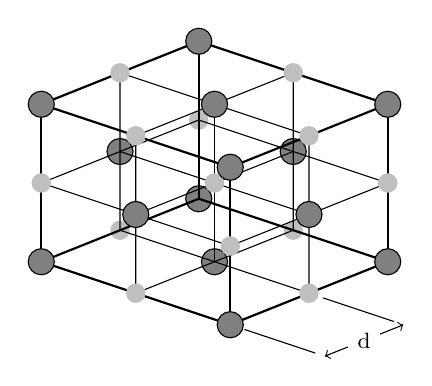
\begin{tikzpicture}[y={(-.6cm,0.2cm)},x={(.5cm,.2cm)}, z={(0cm,.5cm)}]
% coordinate system
\coordinate (O) at (0, 0, 0);
\node[circle,scale=1,fill=gray,draw]at(2,2,0){};
\node[circle,scale=1,fill=gray,draw]at(2,0,2){};
\node[circle,scale=1,fill=gray,draw]at(0,2,2){};
\node[circle,scale=1,fill=gray,draw]at(0,0,0){};
\node[circle,scale=.7,fill=lightgray,draw=lightgray]at(2,2,2){};
\node[circle,scale=.7,fill=lightgray,draw=lightgray]at(2,0,0){};
\node[circle,scale=.7,fill=lightgray,draw=lightgray]at(0,2,0){};
%bonds
\draw[thick](-2,-2,0)--(-2,2,0)--(2,2,0)--(2,-2,0)--cycle;
\draw[thick](-2,-2,4)--(-2,2,4)--(2,2,4)--(2,-2,4)--cycle;
\draw[thick](-2,-2,0)--(-2,-2,4);
\draw[thick](-2,2,0)--(-2,2,4);
\draw[thick](2,-2,0)--(2,-2,4);
\draw[thick](2,2,0)--(2,2,4);
\draw[](-2,-2,2)--(-2,2,2)--(2,2,2)--(2,-2,2)--cycle;
\draw[](0,-2,4)--(0,-2,0)--(0,2,0)--(0,2,4)--cycle;
\draw[](-2,0,0)--(-2,0,4)--(2,0,4)--(2,0,0)--cycle;
\draw[](0,-2,2)--(0,2,2);
\draw[](2,0,2)--(-2,0,2);
\draw[](0,0,4)--(0,0,0);
%atoms
\node[circle,scale=.7,fill=lightgray,draw=lightgray]at(0,0,2){};
\node[circle,scale=1,fill=gray,draw]at(-2,-2,0){};
\node[circle,scale=1,fill=gray,draw]at(2,-2,0){};
\node[circle,scale=1,fill=gray,draw]at(-2,2,0){};
\node[circle,scale=1,fill=gray,draw]at(2,2,4){};
\node[circle,scale=1,fill=gray,draw]at(2,-2,4){};
\node[circle,scale=1,fill=gray,draw]at(-2,2,4){};
\node[circle,scale=1,fill=gray,draw]at(-2,-2,4){};
\node[circle,scale=1,fill=gray,draw]at(0,-2,2){};
\node[circle,scale=1,fill=gray,draw]at(-2,0,2){};
\node[circle,scale=1,fill=gray,draw]at(0,0,4){};
\node[circle,scale=.7,fill=lightgray,draw=lightgray]at(-2,0,0){};
\node[circle,scale=.7,fill=lightgray,draw=lightgray]at(0,-2,0){};
\node[circle,scale=.7,fill=lightgray,draw=lightgray]at(-2,0,4){};
\node[circle,scale=.7,fill=lightgray,draw=lightgray]at(0,-2,4){};
\node[circle,scale=.7,fill=lightgray,draw=lightgray]at(0,2,4){};
\node[circle,scale=.7,fill=lightgray,draw=lightgray]at(2,0,4){};
\node[circle,scale=.7,fill=lightgray,draw=lightgray]at(-2,2,2){};
\node[circle,scale=.7,fill=lightgray,draw=lightgray]at(2,-2,2){};
\node[circle,scale=.7,fill=lightgray,draw=lightgray]at(-2,-2,2){};
%label
\draw[<->](0,-4,0)--(-2,-4,0);
\draw[](0,-2.3,0)--(0,-3.8,0);
\draw[](-2,-2.3,0)--(-2,-3.8,0);
\node[font=\footnotesize,fill=white]at(-1,-4,0){d};
\end{tikzpicture}
\caption{Crystalline structure of a Lithium Fluoride.}
\label{fig:xr5}
\end{figure}







\newpage
\section{Copying and pasting elements}



\begin{figure}
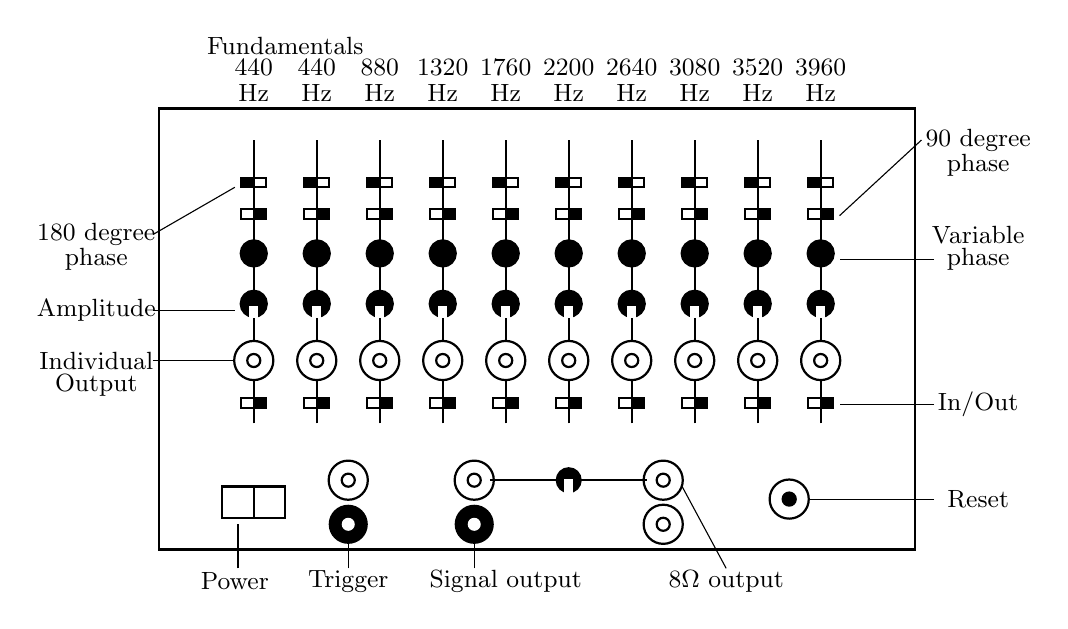
\begin{tikzpicture}[thick,scale=.8,font=\small]
\draw(0,0)rectangle(12,7); %box
\foreach \x in {0,1,2,3,4,5,6,7,8,9}
{
\begin{scope}[shift={(.5,0)}]
%dials
\draw(1+\x,2)--(1+\x,6.5);
\node[black,fill=white,draw=black,shape=circle,scale=1.5] at (1+\x,3){};
\node[black,fill=white,draw=black,shape=circle,scale=.5] at (1+\x,3){};
\draw(.8+\x,2.25)rectangle(1+\x,2.4);
\draw[fill=black](1+\x,2.25)rectangle(1.2+\x,2.4);
\node[black,fill=black,draw=black,shape=circle,scale=1] at (1+\x,3.9){};
\node[black,fill=black,draw=black,shape=circle,scale=1] at (1+\x,4.7){};
\draw(.8+\x,5.25)rectangle(1+\x,5.4);
\draw[fill=black](1+\x,5.25)rectangle(1.2+\x,5.4);
\draw[fill=black](.8+\x,5.75)rectangle(1+\x,5.9);
\draw[fill=white](1+\x,5.75)rectangle(1.2+\x,5.9);
\draw[fill=white,draw=white](.95+\x,3.7)rectangle(1.05+\x,3.85);
\node at (1+\x,7.25){Hz};
\end{scope}
}
\draw(1,.5)rectangle(2,1);
\draw(1.5,.5)--(1.5,1);
\node[fill=black,shape=circle,scale=1.5] at (3,.4){}; %trigger
\node[fill=white,shape=circle,scale=.5] at (3,.4){}; %trigger
\node[draw=black,fill=white,shape=circle,scale=1.5] at (3,1.1){};
\node[draw=black,fill=white,shape=circle,scale=.5] at (3,1.1){};
\node[fill=black,shape=circle,scale=1.5] at (5,.4){}; %signal output
\node[fill=white,shape=circle,scale=.5] at (5,.4){}; %signal output
\node[draw=black,fill=white,shape=circle,scale=1.5] at (5,1.1){}; %8ohm output
\node[draw=black,fill=white,shape=circle,scale=.5] at (5,1.1){}; %8ohm output
\node[draw=black,fill=white,shape=circle,scale=1.5] at (8,1.1){}; %8ohm output
\node[draw=black,fill=white,shape=circle,scale=.5] at (8,1.1){}; %8ohm output
\node[draw=black,fill=white,shape=circle,scale=1.5] at (8,.4){}; %8ohm output
\node[draw=black,fill=white,shape=circle,scale=.5] at (8,.4){}; %8ohm output
\node[draw=black,fill=white,shape=circle,scale=1.5] at (10,.8){}; %reset
\node[draw=black,fill=black,shape=circle,scale=.5] at (10,.8){}; %reset
\draw(5.25,1.1)--(7.75,1.1);
\node[fill=black,shape=circle,scale=1] at (6.5,1.1){};
\draw[fill=white,draw=white](6.45,.9)rectangle(6.55,1.1);
%labels
\node at (2,8){Fundamentals};
\node at (1.5,7.65){440};
\node at (2.5,7.65){440};
\node at (3.5,7.65){880};
\node at (4.5,7.65){1320};
\node at (5.5,7.65){1760};
\node at (6.5,7.65){2200};
\node at (7.5,7.65){2640};
\node at (8.5,7.65){3080};
\node at (9.5,7.65){3520};
\node at (10.5,7.65){3960};
\node at (-1,5){180 degree};
\node at (-1,4.6){phase};
\draw[thin](-.1,5)--(1.2,5.75);
\node at (-1,3.8){Amplitude};
\draw[thin](-.1,3.8)--(1.2,3.8);
\node at (-1,3){Individual};
\node at (-1,2.6){Output};
\draw[thin](-.1,3)--(1.2,3);
\node at (13,6.5){90 degree};
\node at (13,6.1){phase};
\draw[thin](12.1,6.5)--(10.8,5.3);
\node at (13,5){Variable};
\node at (13,4.6){phase};
\draw[thin](12.3,4.6)--(10.8,4.6);
\node at (13,2.3){In/Out};
\draw[thin](12.3,2.3)--(10.8,2.3);
\node at (13,.8){Reset};
\draw[thin](12.3,.8)--(10.3,.8);
\node at (9,-.5){8$\Omega$ output};
\draw[thin](9,-.3)--(8.3,1);
\node at (5.5,-.5){Signal output};
\draw[thin](5,-.3)--(5,.1);
\node at (3,-.5){Trigger};
\draw[thin](3,-.3)--(3,.1);
\node at (1.2,-.5){Power};
\draw[thin](1.25,-.3)--(1.25,.4);
\end{tikzpicture}
\caption{A Fourier synthesizer.}
\label{fig:fs4}
\end{figure}





\newpage
\section{Circuit diagrams}








\newpage
\section{Drawing on top of images}

\begin{figure}
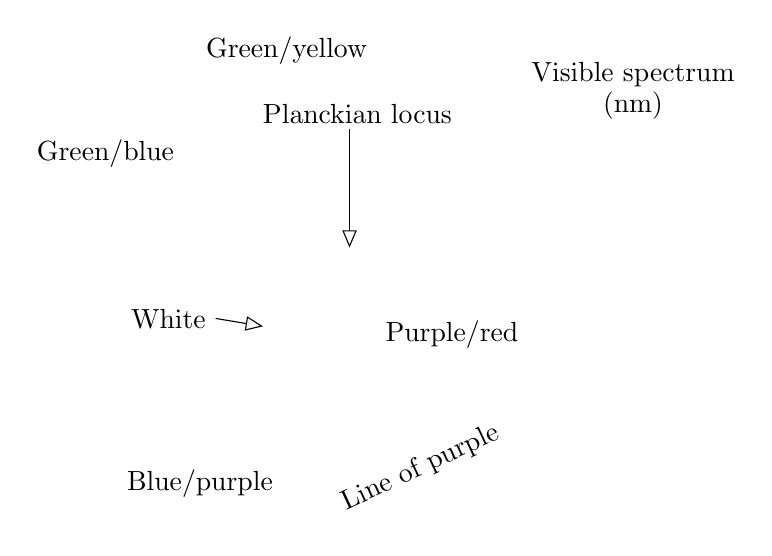
\begin{tikzpicture}

%\node[above right]at(0,0){\includegraphics[scale=.24]{/usr/local/master/labs/physics325-WI2017/Colour-Temperature/chromaticityDiagram.png}};
\node[]at(4.6,8.2){Green/yellow};
\node[]at(2.3,6.9){Green/blue};
\node[]at(3.1,4.8){White};
\draw[-open triangle 45](3.7,4.8)--(4.3,4.7);
\node[]at(5.5,7.4){Planckian locus};
\draw[-open triangle 45](5.4,7.2)--(5.4,5.7);
\node[]at(9,7.9){Visible spectrum};
\node[]at(9,7.5){(nm)};
\node[]at(6.7,4.6){Purple/red};
\node[rotate=25]at(6.3,2.9){Line of purple};
\node[]at(3.5,2.7){Blue/purple};

\end{tikzpicture}
  \caption{Chromaticity diagram}
  \label{fig:ctChromaticityDiagram}
\end{figure}





\newpage
\section{Cables, tubes, and pipes}


\begin{figure}
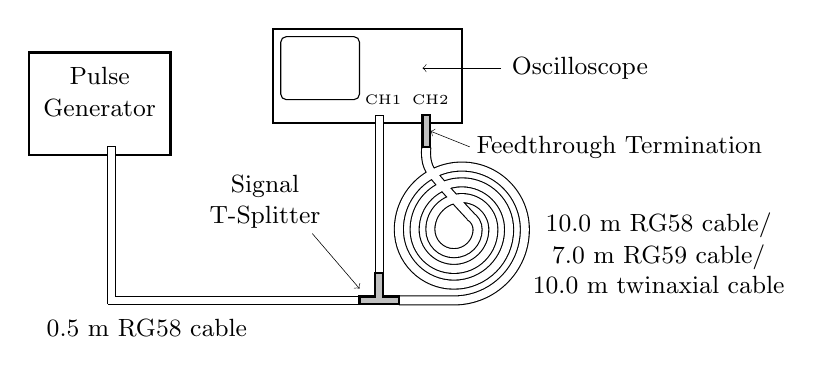
\begin{tikzpicture}
\draw[thick](0,1.9)rectangle(1.8,3.2); %pulse generator
\draw[thin,fill=white](1,0)--(4.2,0)--(4.2,.1)--(1.1,.1)--(1.1,2)--(1,2)--(1,0); %cable
\draw[double distance=.1cm](4.7,.05)--(5.4,.05)arc(270:360:.9)arc(0:180:.8)arc(180:360:.7)
arc(0:180:.6)arc(180:360:.5)arc(0:180:.4)arc(180:360:.3)arc(0:60:.2) 
plot [smooth] coordinates {(5.62,1.11) (5.1,1.7) (5.05,2)}; %cable to be tested
\draw[thick,fill=white](3.1,2.3)rectangle(5.5,3.5); %oscilloscope
\draw[rounded corners=2pt](3.2,2.6)rectangle(4.2,3.4); %oscilloscope screen
\draw[fill=lightgray,thick](5,2)rectangle(5.1,2.4); %feedthrough to CH2
\draw[fill=white](4.4,.2)rectangle(4.5,2.4); %to CH1
\draw[thick,fill=lightgray](4.2,.1)--(4.4,.1)--(4.4,.4)--(4.5,.4)--(4.5,.1)--(4.7,.1)--(4.7,0)
--(4.2,0)--cycle; %splitter
%labels
\node[font=\small]at(7,3){Oscilloscope};
\draw[very thin,->](6,3)--(5,3);
\node[font=\small]at(7.5,2){Feedthrough Termination};
\draw[very thin,->](5.6,2)--(5.1,2.2);
\node[font=\tiny]at(5.1,2.6){CH2};
\node[font=\tiny]at(4.5,2.6){CH1};
\node[font=\small]at(8,1){10.0 m RG58 cable/};
\node[font=\small]at(8,.6){7.0 m RG59 cable/};
\node[font=\small]at(8.,.25){10.0 m twinaxial cable};
\node[font=\small]at(3,1.5){Signal};
\node[font=\small]at(3,1.1){T-Splitter};
\draw[very thin,->](3.6,.9)--(4.2,.2);
\node[font=\small]at(1.5,-.3){0.5 m RG58 cable};
\node[font=\small]at(.9,2.9){Pulse};
\node[font=\small]at(.9,2.5){Generator};
\end{tikzpicture}
\caption{A diagram of the experimental set up for the determination of signal attenuation in RG58, RG59, and twinaxial cables.}
\label{fig:tw2}
\end{figure}



%%%%%%%%%%%%%
\AtEndDocument{\clearpage\ifodd\value{page}\else\null\clearpage\fi}
% forces even page count, for double sided printing 

%%%end companion guide%%% DO NOT REMOVE THIS LINE

\end{document}
